\documentclass[12pt,a4paper]{article}

%% Desactivar shorthands de babel español para evitar conflictos con TikZ
\PassOptionsToPackage{es-noshorthands}{babel}
\usepackage{formato}

%% Paquetes adicionales para el contenido
\usepackage{pgfgantt}
\usepackage{mdframed}
\usepackage{siunitx}
\usepackage{longtable}
\usepackage{tabularx}

%% Colores personalizados
\definecolor{unsaacRed}{RGB}{155,27,48}
\definecolor{unsaacGray}{RGB}{90,90,90}
\definecolor{lightGray}{RGB}{245,245,245}
\definecolor{accent}{RGB}{200,50,70}

%% TikZ librerías adicionales
\usetikzlibrary{shapes,arrows}

%% Nuevos tipos de columna
\newcolumntype{C}[1]{>{\centering\arraybackslash}p{#1}}
\newcolumntype{L}[1]{>{\raggedright\arraybackslash}p{#1}}
\newcolumntype{R}[1]{>{\raggedleft\arraybackslash}p{#1}}

%% Entorno supuesto (mdframed)
\newmdenv[
  backgroundcolor=lightGray,
  linecolor=unsaacGray,
  linewidth=0.5pt,
  innerleftmargin=8pt,
  innerrightmargin=8pt,
  innertopmargin=6pt,
  innerbottommargin=6pt,
  skipabove=6pt,
  skipbelow=6pt
]{supuesto}

%% Siunitx
\sisetup{output-decimal-marker={,}}

%% =====================================================
%% CONFIGURACIÓN DE LOS DATOS DEL DOCUMENTO
%% =====================================================
\documenttitle{Plataforma Web para la Optimización de la Gestión del TUPA de la UNSAAC}
\subject{Desarrollo de Software I}
\advisor{Mg. Luis Alvaro Monzón Condori}
\semester{2026 - I}

%% =====================================================
%% REGISTRO DE AUTORES/ESTUDIANTES
%% =====================================================
\addauthor{Castro Pari, Rayneld Fidel}{231865}
\addauthor{Estacio Medrano, Amilcar}{200822}
\addauthor{Florez Vega, Yamir Wagner}{231442}
\addauthor{Merma Ccarhuarupay, Adel Alejandro}{231446}

%% =====================================================
%% INICIO DEL DOCUMENTO
%% =====================================================
\begin{document}

%% PORTADA
\thispagestyle{empty}
\makeatletter
%% =====================================================
%% Portada - Documento académico - Versión APA
%% =====================================================
\makeatletter
\begin{titlepage}
    \thispagestyle{empty}

    \singlespacing

    %% =====================================================
    %% ENCABEZADO INSTITUCIONAL
    %% =====================================================
    \begin{center}
        UNIVERSIDAD NACIONAL DE SAN ANTONIO ABAD DEL CUSCO\\[0.3cm]
        FACULTAD DE INGENIERÍA ELÉCTRICA, ELECTRÓNICA, INFORMÁTICA Y MECÁNICA\\[0.3cm]
        ESCUELA PROFESIONAL DE INGENIERÍA INFORMÁTICA Y DE SISTEMAS
    \end{center}

    %% =====================================================
    %% ESCUDO/LOGO INSTITUCIONAL
    %% =====================================================
    \vspace{0.25cm}
    \begin{figure}[H]
        \centering
        
\includegraphics[scale=0.25]{images/Logo-UNSAAC.png}
        \hspace{1cm}
        
\includegraphics[scale=0.25]{images/Logo-Informatica.png}
    \end{figure}

    %% =====================================================
    %% TÍTULO DEL DOCUMENTO
    %% =====================================================
    \begin{center}
        \rule{\linewidth}{0.6mm} \\[0.3cm]
        {\large \textbf{\@documenttitle}} \\[0.1cm]
        \rule{\linewidth}{0.6mm}
    \end{center}

    \vspace{0.5cm}

    %% =====================================================
    %% INFORMACIÓN DEL CURSO Y PARTICIPANTES
    %% =====================================================
    \noindent\hspace*{1.5cm}%
    \parbox{0.85\textwidth}{
        \raggedright
        \textbf{Asignatura:} \\
        \hspace*{1em} \@subject \\[0.8cm]
        \textbf{Docente:} \\
        \hspace*{1em} \@advisor \\[0.8cm]
        \textbf{Estudiantes:} \\
        \hspace*{1em}
        \parbox{\dimexpr\linewidth-2em\relax}{
            \vspace{0.5em}
            \begin{tabular}{l@{\hspace{2em}}l}
                \authorlist
            \end{tabular}
        }
    }

    \vfill

    %% =====================================================
    %% FECHA DE PUBLICACIÓN
    %% =====================================================
    \begin{center}
        Cusco - Perú \\ \the\year
    \end{center}

\end{titlepage}
\doublespacing
\makeatother
\newpage

\makeatother

%% SECCIONES PRELIMINARES CON NUMERACIÓN ROMANA
\startpreliminary
\clearpage

%% TABLA DE CONTENIDOS
\tableofcontents
\clearpage

%% CONTENIDO PRINCIPAL CON NUMERACIÓN ARÁBIGA
\startmain

% ── Presentación ─────────────────────────────────────────────────────────────
\section{Presentación}

El presente documento constituye el Plan de Proyecto correspondiente al primer
entregable semestral del curso de Ingeniería de Software, desarrollado por un equipo
de la Escuela Profesional de Ingeniería Informática y de Sistemas de la Universidad
Nacional de San Antonio Abad del Cusco (UNSAAC).

El proyecto tiene como propósito el diseño y desarrollo de una \textbf{Plataforma Web
para la Optimización de la Gestión del TUPA de la UNSAAC}, entendiendo el TUPA
(\emph{Texto Único de Procedimientos Administrativos}) como el instrumento de gestión
institucional que concentra la totalidad de procedimientos administrativos y servicios
prestados por la universidad, junto con sus requisitos, costos, plazos, bases legales
y unidades orgánicas responsables.

Este plan articula la justificación del problema identificado, los objetivos de la
solución propuesta, la metodología de trabajo adoptada, los recursos necesarios, el
cronograma de ejecución, el presupuesto estimado y la descripción del prototipado
dinámico planificado. Su elaboración sigue los principios de la Ingeniería de
Requerimientos y responde a los lineamientos del atributo de graduado AG-C12, con
énfasis particular en la capacidad de adquirir y formular especificaciones de software
de manera sistemática y fundamentada (AG-C12.01).

\begin{supuesto}
\small\textbf{Nota:} Los datos de integrantes y docente deben completarse con la
información real del equipo antes de la entrega formal. Los supuestos asumidos a lo
largo del informe se indican explícitamente en recuadros de este estilo.
\end{supuesto}


\section{Ámbito de Aplicación o Influencia}
 
\subsection{Descripción del ámbito}
 
El proyecto está orientado al entorno administrativo y académico de la \textbf{Universidad Nacional de San Antonio Abad del Cusco (UNSAAC)}, específicamente en los procesos relacionados con la gestión de los procedimientos establecidos en el Texto Único de Procedimientos Administrativos (TUPA).
 
La propuesta se desarrolla dentro del contexto de la \textbf{transformación digital universitaria}, buscando modernizar los servicios administrativos mediante el uso de tecnologías web que permitan automatizar procesos, mejorar la atención a los usuarios y optimizar el control y seguimiento de expedientes administrativos.
 
\subsection{Ámbito institucional}
 
El proyecto tiene como ámbito de aplicación directo la UNSAAC, con sede principal en Cusco y filiales en:
 
\begin{itemize}[noitemsep]
    \item Cusco (Sede Central)
    \item Sicuani
    \item Espinar
    \item Puerto Maldonado
    \item Santo Tomás
    \item Yanaoca
    \item Andahuaylas
\end{itemize}
 
El sistema PLADDES (\textit{tramite.unsaac.edu.pe}) es la plataforma oficial de trámite documentario virtual de la institución y es el objeto de mejora de este proyecto.
 
\subsection{Área de influencia}
 
Entre las principales unidades involucradas se encuentran:
 
\begin{itemize}[noitemsep]
    \item Rectorado
    \item Vicerrectorado Académico
    \item Decanatos de Facultad
    \item Escuela de Posgrado
    \item Centro de Cómputo
    \item Oficina de Admisión
    \item Mesa de Partes Virtual
    \item Unidades de Trámite Documentario
\end{itemize}
 
\subsection{Usuarios objetivo / Beneficiarios}
 
\begin{itemize}
    \item \textbf{Estudiantes de pregrado y posgrado:} principal grupo que registra solicitudes en PLADDES para trámites como certificados, constancias, homologaciones, grado y título, entre otros.
    \item \textbf{Docentes y personal cesante/administrativo:} usuarios que gestionan trámites propios de su condición laboral a través del sistema.
    \item \textbf{Dependencias administrativas:} Unidad de Trámite Documentario, Decanatos, Escuelas Profesionales, VRAC, DIGA, UTH, SG y demás oficinas que reciben y resuelven los expedientes ingresados en PLADDES.
    \item \textbf{Público en general e instituciones:} personas externas a la comunidad universitaria que acceden a servicios puntuales del TUPA.
    \item \textbf{La institución universitaria en general,} que se verá favorecida con el fortalecimiento de la modernización administrativa y la mejora en la calidad del servicio.
\end{itemize}
 
\subsection{Alcance funcional}
 
El proyecto rediseña y optimiza los flujos existentes en PLADDES, abarcando:
 
\begin{enumerate}
    \item \textbf{Registro de solicitudes:} el wizard de 4 pasos actual será reemplazado por un flujo moderno, guiado e intuitivo.
    \item \textbf{Catálogo de trámites TUPA:} presentación clara de los 80+ procedimientos con requisitos, costos, plazos y canales de atención, integrada al flujo de registro.
    \item \textbf{Seguimiento de expedientes:} mejora del módulo de consulta de estado de trámite con vista de línea de tiempo y notificaciones.
    \item \textbf{Gestión de pagos:} integración mejorada del proceso de verificación de voucher de pago, actualmente manual.
    \item \textbf{Panel administrativo:} rediseño del panel de las dependencias para gestión eficiente de la bandeja de expedientes.
    \item \textbf{Reportes y estadísticas:} módulo nuevo para generación de reportes de trámites procesados por dependencia y período.
\end{enumerate}
\section{Descripción de la Problemática}
 
\subsection{Situación actual}
 
Actualmente, la gestión de los procedimientos administrativos establecidos en el TUPA de la UNSAAC presenta diversas limitaciones. El sistema PLADDES fue desarrollado con tecnologías de generación anterior: \textbf{AdminLTE 2 + Bootstrap 3 + jQuery}, frameworks que ya no reciben actualizaciones activas de seguridad ni mejoras de rendimiento.
 
Muchos procesos aún dependen de mecanismos manuales, documentación física y procedimientos descentralizados que dificultan la eficiencia institucional. Los estudiantes, egresados y demás administrados enfrentan constantemente problemas como largas colas, desconocimiento de requisitos, retrasos en la validación documentaria, falta de seguimiento en tiempo real de sus expedientes y poca transparencia respecto al estado de sus trámites.
 
\subsection{Formulación del problema}
 
\textbf{Problema general:} ¿De qué manera una plataforma web transaccional puede optimizar la gestión de los procedimientos administrativos del TUPA de la UNSAAC, mejorando la eficiencia, transparencia y seguimiento de los trámites universitarios?
 
\textbf{Problemas específicos:}
\begin{itemize}
    \item ¿Cómo reducir el tiempo de atención y procesamiento de los trámites administrativos?
    \item ¿Cómo centralizar la información relacionada con requisitos, costos, plazos y estados de los procedimientos del TUPA?
    \item ¿Cómo mejorar el seguimiento y la trazabilidad de los expedientes en tiempo real?
    \item ¿Cómo optimizar la gestión documental y el flujo de trabajo entre las diferentes oficinas?
    \item ¿Cómo implementar mecanismos digitales que disminuyan errores manuales y mejoren la transparencia administrativa?
\end{itemize}
 
\subsection{Problemas identificados en PLADDES}
 
\begin{longtable}{>{\bfseries}p{1.2cm} p{12cm}}
\toprule
\textbf{Cód.} & \textbf{Problema} \\
\midrule
\endhead
P1 & \textbf{Deuda tecnológica acumulada:} el frontend está construido sobre AdminLTE 2 con Bootstrap 3 y jQuery, tecnologías obsoletas desde 2019. Esto dificulta el mantenimiento, la incorporación de nuevas funcionalidades y la corrección de vulnerabilidades de seguridad. \\[0.3cm]
P2 & \textbf{Experiencia de usuario deficiente en el formulario de solicitud:} el proceso de registro se presenta como un wizard de 4 pasos con una interfaz poco intuitiva, sin validación en tiempo real ni mensajes de error claros. \\[0.3cm]
P3 & \textbf{Seguimiento de trámites limitado:} la opción ``Verifique AQUÍ su trámite'' no ofrece vista de línea de tiempo, historial de estados ni información sobre la dependencia responsable en cada momento. \\[0.3cm]
P4 & \textbf{Verificación de pagos manual y sin integración:} el sistema exige adjuntar el voucher de pago, pero no existe verificación automática con los sistemas de caja de la UNSAAC. \\[0.3cm]
P5 & \textbf{Ausencia de notificaciones activas:} el único mecanismo de comunicación es el correo electrónico ingresado manualmente, sin confirmaciones automáticas al registrar ni alertas al cambiar el estado del trámite. \\[0.3cm]
P6 & \textbf{Problemas de disponibilidad:} el sistema muestra avisos del tipo ``NO REALICE NINGÚN TRÁMITE, ESTAMOS EN MANTENIMIENTO'' directamente en la página principal, generando desconfianza. \\[0.3cm]
P7 & \textbf{Catálogo de trámites no integrado:} los requisitos, costos y plazos del TUPA están disponibles únicamente como documento PDF externo, desvinculado del sistema. \\[0.3cm]
P8 & \textbf{Gestión documental sin estándar claro:} el sistema acepta múltiples formatos pero no guía al usuario sobre qué documentos específicos debe adjuntar según el tipo de trámite seleccionado. \\[0.3cm]
P9 & \textbf{Sin panel administrativo de gestión:} las dependencias no cuentan con un panel dedicado para monitorear su bandeja de expedientes pendientes, asignar responsables ni generar reportes de productividad. \\
\bottomrule
\end{longtable}
 
\subsection{Impacto del problema}
 
\begin{itemize}
    \item \textbf{Retrasos en la atención:} trámites observados por documentación incompleta que pudo prevenirse con guía contextual en el formulario.
    \item \textbf{Sobrecarga del personal} de la Unidad de Trámite Documentario por validaciones manuales de pagos y consultas telefónicas de seguimiento.
    \item \textbf{Insatisfacción de la comunidad universitaria,} especialmente de estudiantes de las filiales que dependen exclusivamente del canal virtual.
    \item \textbf{Riesgo de incumplimiento del silencio administrativo positivo} establecido en el TUPA (plazos de 5 a 30 días hábiles según el procedimiento).
    \item \textbf{Imposibilidad de auditar} el desempeño administrativo por ausencia de estadísticas y reportes automatizados.
\end{itemize}
\section{Objetivos de la Propuesta}
 
\subsection{Objetivo General}
 
\begin{quote}
\textit{Rediseñar y optimizar el Sistema PLADDES de Trámite Documentario Virtual de la UNSAAC (\textit{tramite.unsaac.edu.pe}), migrando su arquitectura tecnológica a un stack moderno y mejorando la experiencia de usuario, la integración con el catálogo TUPA, el seguimiento de expedientes y la gestión administrativa; mediante el desarrollo de una plataforma web transaccional que automatice los procedimientos establecidos en el TUPA institucional, mejorando la eficiencia, transparencia y seguimiento de los trámites universitarios.}
\end{quote}
 
\subsection{Objetivos Específicos}
 
\begin{enumerate}
    \item \textbf{Migrar el frontend} de AdminLTE 2/Bootstrap 3/jQuery a \textbf{React.js + Tailwind CSS}, eliminando la deuda tecnológica y mejorando el rendimiento y mantenibilidad del sistema. \textit{(Atiende P1)}
 
    \item \textbf{Rediseñar el flujo de registro de solicitudes} con validación en tiempo real, mensajes de error claros y confirmación de envío explícita para el usuario. \textit{(Atiende P2)}
 
    \item \textbf{Implementar un panel de seguimiento de expedientes} con vista de línea de tiempo, historial de estados y dependencia responsable visible en cada etapa. \textit{(Atiende P3)}
 
    \item \textbf{Desarrollar un módulo de verificación de pagos} que permita al sistema cruzar el código de pago con los registros de caja, reduciendo la validación manual. \textit{(Atiende P4)}
 
    \item \textbf{Implementar notificaciones automáticas por correo electrónico} al registrar una solicitud y en cada cambio de estado del expediente. \textit{(Atiende P5)}
 
    \item \textbf{Establecer un mecanismo formal de gestión de mantenimientos programados} con avisos anticipados y página de estado del servicio. \textit{(Atiende P6)}
 
    \item \textbf{Integrar el catálogo digital del TUPA} (procedimientos, requisitos, costos y plazos) directamente en el flujo de registro, de forma contextual según el tipo de trámite seleccionado. \textit{(Atiende P7)}
 
    \item \textbf{Implementar guía de documentos requeridos} por tipo de trámite, indicando al usuario exactamente qué archivos adjuntar antes de enviar su solicitud. \textit{(Atiende P8)}
 
    \item \textbf{Desarrollar un panel administrativo} para las dependencias (Decanatos, VRAC, DIGA, UTH, etc.) con bandeja de expedientes, asignación de responsables, reportes y estadísticas de productividad. \textit{(Atiende P9)}
\end{enumerate}
\section{Metodología}
% ══════════════════════════════════════════════════════════════════════════════

\subsection{Metodología de desarrollo}

El proyecto adoptará \textbf{Scrum} como marco de trabajo ágil, complementado con
prácticas de \textbf{Ingeniería de Requerimientos} basadas en el estándar IEEE~830
y principios de diseño centrado en el usuario (UCD). Esta combinación permite
gestionar incertidumbre, incorporar retroalimentación continua y entregar valor
incremental a lo largo del ciclo de vida del desarrollo.

La elección de Scrum se fundamenta en el análisis de plataformas de referencia:

\begin{itemize}
  \item \textbf{PLADDES -- UNSAAC} (\texttt{tramite.unsaac.edu.pe}): sistema actual
    de trámite documentario de la UNSAAC que gestiona solicitudes virtuales
    clasificadas por tipo de usuario (estudiante, docente, administrativo, público
    general), seguimiento de expedientes y adjunto de vouchers de pago.
    Constituye el mayor referente directo del proyecto; sus limitaciones de
    usabilidad y ausencia de notificaciones proactivas son el punto de partida
    para las mejoras propuestas.

  \item \textbf{Portal Administrativo -- PUCP}: plataforma que centraliza
    información de trámites paso a paso para toda la comunidad universitaria,
    integra pagos académicos virtuales y ofrece paneles diferenciados por
    dirección. Destaca por su arquitectura orientada a servicios y la
    digitalización progresiva de ventanillas presenciales.

  \item \textbf{SISADES -- Universidad Nacional de Huancavelica}: sistema
    integral que centraliza documentos institucionales, biblioteca virtual y
    seguimiento de egresados. Su mesa de partes virtual y el módulo de
    seguimiento de trámites publicado en la Plataforma del Estado Peruano
    (gob.pe) evidencian una integración con estándares de interoperabilidad
    pública que el presente proyecto también considerará.
\end{itemize}

\subsubsection{Roles Scrum}

\begin{center}
\begin{tabular}{p{3.5cm} p{9.5cm}}
  \toprule
  \rowcolor{unsaacRed}
  \color{white}\textbf{Rol} & \color{white}\textbf{Responsabilidad} \\
  \midrule
  Product Owner   & Define y prioriza el \textit{Product Backlog} en función de los
                    objetivos del TUPA y las necesidades de estudiantes y personal
                    administrativo. \\
  Scrum Master    & Facilita ceremonias, elimina impedimentos y asegura que el equipo
                    siga el marco de trabajo. \\
  Dev Team        & Diseña, implementa y prueba los incrementos de producto en cada
                    sprint. \\
  \bottomrule
\end{tabular}
\end{center}

\subsubsection{Ceremonias y artefactos}

\begin{itemize}
  \item \textbf{Sprint Planning}: primera sesión del sprint; se seleccionan ítems
    del backlog y se define el \textit{Sprint Goal}.
  \item \textbf{Daily Stand-up} (10\,min): sincronización diaria de avances,
    impedimentos y planes del día.
  \item \textbf{Sprint Review}: demostración del incremento al \textit{Product
    Owner} y recogida de retroalimentación.
  \item \textbf{Sprint Retrospective}: mejora continua del proceso.
  \item \textbf{Artefactos}: Product Backlog, Sprint Backlog, Definition of Done
    e Incremento potencialmente entregable.
\end{itemize}

\subsubsection{Stack tecnológico propuesto}

\begin{center}
\begin{tabular}{p{3.8cm} p{4.2cm} p{5cm}}
  \toprule
  \rowcolor{unsaacRed}
  \color{white}\textbf{Capa} & \color{white}\textbf{Tecnología} &
  \color{white}\textbf{Justificación} \\
  \midrule
  Frontend        & React.js + Tailwind CSS  & SPA reactiva, ecosistema maduro,
                                               facilita prototipos interactivos. \\
  Backend         & Node.js + Express.js     & API REST ligera, JSON nativo,
                                               alto rendimiento para I/O. \\
  Base de datos   & PostgreSQL               & Soporte robusto de relaciones,
                                               transacciones y consultas complejas. \\
  Autenticación   & JWT + OAuth2             & Seguridad estándar para sesiones
                                               y roles diferenciados. \\
  Notificaciones  & Nodemailer + WebSockets  & Alertas por correo y en tiempo
                                               real sobre estado de trámites. \\
  Control de versiones & Git + GitHub        & Flujo colaborativo con ramas por
                                               feature y pull requests. \\
  Contenerización & Docker / Docker Compose  & Entornos reproducibles para
                                               desarrollo y despliegue. \\
  \bottomrule
\end{tabular}
\end{center}

% ──────────────────────────────────────────────────────────────────────────────
\subsection{Actividades principales}

El proyecto se organiza en \textbf{cuatro sprints} de dos semanas cada uno, más
una fase inicial de planificación (\textit{Sprint 0}), alineados con las dos
entregas formales del semestre.

\subsubsection{Sprint 0 -- Planificación y análisis de requerimientos\\(hasta 28/05/2026 -- Entrega~1)}

\begin{itemize}
  \item Revisión y análisis de la plataforma PLADDES--UNSAAC vigente.
  \item Estudio comparativo de los sistemas de referencia (PUCP, UNH).
  \item Levantamiento de requerimientos funcionales y no funcionales mediante
    entrevistas con usuarios representativos (estudiantes, administrativos).
  \item Elaboración del \textit{Product Backlog} con historias de usuario
    priorizadas (MoSCoW).
  \item Diseño de la arquitectura lógica y física del sistema.
  \item \textbf{Diseño de la base de datos}: modelo entidad-relación y diagrama
    relacional (PostgreSQL).
  \item \textbf{Prototipado dinámico} de las interfaces principales (Figma):
    pantalla de consulta del TUPA, registro de trámite, seguimiento de
    expediente y panel administrativo.
  \item Configuración del repositorio GitHub con estrategia de ramificación
    (\textit{Git Flow}).
  \item Redacción del Plan de Proyecto (presente documento).
\end{itemize}

\subsubsection{Sprint 1 -- Módulo de consulta TUPA e interfaz base
(01/06/2026 -- 12/06/2026)}

\begin{itemize}
  \item Implementación del módulo de \textbf{consulta de procedimientos}: listado,
    búsqueda por categoría, detalle de requisitos y costos asociados del TUPA.
  \item Desarrollo de la \textbf{autenticación y gestión de usuarios}: registro,
    inicio de sesión, roles (estudiante, administrativo, administrador).
  \item Construcción del \textbf{layout base} de la aplicación: barra de
    navegación, footer, diseño responsivo y sistema de estilos.
  \item Configuración del entorno de base de datos y migraciones iniciales.
  \item Pruebas unitarias de los endpoints REST y pruebas de usabilidad del
    módulo de consulta.
\end{itemize}

\subsubsection{Sprint 2 -- Módulo de registro y seguimiento de trámites
(15/06/2026 -- 26/06/2026)}

\begin{itemize}
  \item Implementación del \textbf{formulario de registro de trámite}: datos del
    solicitante, selección de procedimiento TUPA, adjunto de documentos digitales
    y clave de pago.
  \item Desarrollo del \textbf{módulo de seguimiento de expedientes}: estado
    actual, historial de movimientos y observaciones por oficina.
  \item \textbf{Sistema de notificaciones}: alertas por correo electrónico ante
    cambios de estado (recibido, en revisión, observado, resuelto).
  \item Validación digital de documentos adjuntos (tipo, tamaño, formato PDF).
  \item Pruebas de integración del flujo completo de registro y seguimiento.
\end{itemize}

\subsubsection{Sprint 3 -- Panel administrativo y módulo de reportes
(29/06/2026 -- 10/07/2026)}

\begin{itemize}
  \item Desarrollo del \textbf{panel de control administrativo}: bandeja de
    trámites recibidos, cambio de estado, asignación a oficina responsable y
    registro de observaciones.
  \item Implementación del \textbf{módulo de reportes y estadísticas}: trámites
    procesados por período, tiempo de atención promedio, procedimientos más
    solicitados y exportación a PDF/Excel.
  \item Mejoras de \textbf{accesibilidad} (WCAG 2.1 nivel AA): contraste,
    etiquetas ARIA, navegación por teclado.
  \item Pruebas de carga y rendimiento básicas.
\end{itemize}

\subsubsection{Sprint 4 -- Integración, pruebas finales y documentación
(13/07/2026 -- primera semana de agosto 2026 -- Entrega 2)}

\begin{itemize}
  \item Integración de todos los módulos y pruebas de regresión del sistema.
  \item Corrección de defectos identificados en sprints anteriores.
  \item Despliegue de la versión de demostración en entorno de pruebas (Docker).
  \item Elaboración de la \textbf{documentación técnica}: diagramas de
    arquitectura, manual de usuario, diccionario de datos y guía de instalación.
  \item Actualización del repositorio GitHub con commits organizados por módulo.
  \item Preparación de la \textbf{demostración funcional} de la plataforma
    (Entrega Semestral N.º 2, primera semana de agosto de 2026).
\end{itemize}

% ──────────────────────────────────────────────────────────────────────────────
\subsection{Infraestructura y recursos}

\subsubsection{Hardware}

\begin{center}
\begin{tabular}{p{4.5cm} p{4cm} p{4.5cm}}
  \toprule
  \rowcolor{unsaacRed}
  \color{white}\textbf{Recurso} & \color{white}\textbf{Especificación mínima} &
  \color{white}\textbf{Uso} \\
  \midrule
  Laptops de desarrollo   & 8\,GB RAM, CPU i5/Ryzen 5, SSD 256\,GB &
                            Desarrollo y pruebas locales. \\
  Servidor de despliegue  & VPS 2\,vCPU, 4\,GB RAM, 40\,GB SSD     &
                            Entorno de pruebas y demo. \\
  Red universitaria       & Conexión a internet estable              &
                            Acceso a repositorios y herramientas cloud. \\
  \bottomrule
\end{tabular}
\end{center}

\subsubsection{Software y servicios}

\begin{center}
\begin{tabular}{p{4cm} p{3.5cm} p{5.5cm}}
  \toprule
  \rowcolor{unsaacRed}
  \color{white}\textbf{Herramienta} & \color{white}\textbf{Tipo} &
  \color{white}\textbf{Propósito} \\
  \midrule
  Visual Studio Code      & IDE               & Desarrollo del frontend y backend. \\
  Node.js v20 LTS         & Runtime           & Ejecución del servidor Express. \\
  React.js v18            & Framework UI      & Construcción de la SPA. \\
  PostgreSQL 16           & SGBD              & Persistencia de datos. \\
  Docker Desktop          & Contenerización   & Entornos de desarrollo homogéneos. \\
  GitHub                  & Repositorio       & Control de versiones y CI básico. \\
  Figma                   & Diseño UX/UI      & Prototipado dinámico. \\
  Postman                 & Pruebas API       & Validación de endpoints REST. \\
  Trello / Jira (libre)   & Gestión ágil      & Tablero Scrum y seguimiento de tareas. \\
  Nodemailer + SMTP       & Notificaciones    & Envío de alertas por correo. \\
  \bottomrule
\end{tabular}
\end{center}

\subsubsection{Recursos humanos}

El equipo de desarrollo está conformado por \textbf{4 estudiantes} de la
Escuela Profesional de Ingeniería Informática y de Sistemas de la UNSAAC,
quienes asumirán de manera rotativa los roles de \textit{Product Owner},
\textit{Scrum Master} y miembros del \textit{Development Team}.

Como equipo externo de apoyo se contempla la participación de:
\begin{itemize}
  \item \textbf{Docentes asesores} de la asignatura, en calidad de
    \textit{stakeholders} y revisores de entregables.
  \item \textbf{Personal administrativo de la UNSAAC} (muestra representativa)
    para validación de requerimientos y pruebas de usabilidad.
  \item \textbf{Estudiantes voluntarios} para pruebas funcionales y de
    accesibilidad.
\end{itemize}

% ──────────────────────────────────────────────────────────────────────────────
\subsection{Evaluación y monitoreo}

\subsubsection{Mecanismos de control de calidad}

\begin{itemize}
  \item \textbf{Revisión de código} (\textit{Code Review}): toda funcionalidad
    se integra a la rama principal mediante \textit{pull requests} revisados por
    al menos un compañero de equipo antes de aprobar el merge.
  \item \textbf{Definition of Done (DoD)}: un ítem del backlog se considera
    terminado cuando cuenta con código funcional, pruebas unitarias aprobadas,
    documentación básica actualizada y revisión de pares completada.
  \item \textbf{Pruebas unitarias e integración}: uso de \textit{Jest} para el
    backend y \textit{React Testing Library} para el frontend, con cobertura
    mínima del 70\,\% en módulos críticos.
  \item \textbf{Pruebas de usabilidad}: al menos una sesión de prueba con usuarios
    reales por sprint, utilizando la \textit{Escala de Usabilidad del Sistema}
    (SUS) para medir la experiencia de usuario.
\end{itemize}

\subsubsection{Seguimiento del progreso}

\begin{itemize}
  \item \textbf{Tablero Scrum}: visualización del estado de las tareas
    (\textit{To Do} / \textit{In Progress} / \textit{Done}) actualizado
    diariamente.
  \item \textbf{Burndown Chart}: gráfica de trabajo restante vs. tiempo para
    cada sprint, utilizada en la \textit{Sprint Review} para medir la velocidad
    del equipo.
  \item \textbf{Commits en GitHub}: historial versionado que refleja el avance
    diario; se revisará el número de commits y la cobertura de las historias
    de usuario en cada entrega formal.
  \item \textbf{Bitácora de sprints}: documento que registra impedimentos,
    decisiones técnicas y lecciones aprendidas tras cada retrospectiva.
\end{itemize}

\subsubsection{Indicadores de desempeño (KPIs)}

\begin{center}
\begin{tabular}{p{5.5cm} p{3cm} p{4.5cm}}
  \toprule
  \rowcolor{unsaacRed}
  \color{white}\textbf{Indicador} & \color{white}\textbf{Meta} &
  \color{white}\textbf{Herramienta de medición} \\
  \midrule
  Cobertura de pruebas unitarias   & $\geq$ 70\,\%      & Jest / Coverage report \\
  Puntuación SUS (usabilidad)      & $\geq$ 68 puntos   & Cuestionario SUS \\
  Historias completadas por sprint & $\geq$ 80\,\%      & Burndown chart \\
  Tiempo de respuesta de la API    & $\leq$ 500\,ms     & Postman / logs \\
  Defectos críticos en entrega     & 0                  & Registro de bugs (GitHub Issues) \\
  Commits por sprint               & $\geq$ 20          & GitHub insights \\
  \bottomrule
\end{tabular}
\end{center}

\subsubsection{Cronograma de sprints}

\begin{figure}[H]
\centering
\begin{ganttchart}[
    hgrid,
    vgrid,
    x unit=0.46cm,
    y unit title=0.6cm,
    y unit chart=0.55cm,
    title label font=\scriptsize,
    bar label font=\scriptsize,
    bar/.style={fill=unsaacRed!70},
    bar incomplete/.style={fill=unsaacGray!40},
    milestone/.style={fill=unsaacRed, shape=diamond, inner sep=1.5pt},
    today=10,
    today rule/.style={draw=unsaacRed, ultra thick},
    title height=1
  ]{1}{22}
  \gantttitle{Mayo}{2}
  \gantttitle{Junio}{9}
  \gantttitle{Julio}{9}
  \gantttitle{Ago}{2} \\
  \gantttitle{S4}{1}\gantttitle{S5}{1}
  \gantttitle{S1}{1}\gantttitle{S2}{1}\gantttitle{S3}{1}\gantttitle{S4}{1}
  \gantttitle{S1}{1}\gantttitle{S2}{1}\gantttitle{S3}{1}
  \gantttitle{S1}{1}\gantttitle{S2}{1}\gantttitle{S3}{1}\gantttitle{S4}{1}
  \gantttitle{S5}{1}\gantttitle{S1}{1}\gantttitle{S2}{1}\gantttitle{S3}{1}
  \gantttitle{S4}{1}\gantttitle{S5}{1}
  \gantttitle{S1}{1}\gantttitle{S2}{1}\gantttitle{S3}{1} \\
  % Sprint 0
  \ganttbar{Sprint 0: Análisis y planif.}{1}{2} \\
  \ganttmilestone{Entrega 1 (28/05)}{2} \\
  % Sprint 1
  \ganttbar{Sprint 1: Consulta TUPA}{3}{6} \\
  % Sprint 2
  \ganttbar{Sprint 2: Registro/seguim.}{7}{10} \\
  % Sprint 3
  \ganttbar{Sprint 3: Panel admin.}{11}{14} \\
  % Sprint 4
  \ganttbar{Sprint 4: Integración/doc.}{15}{21} \\
  \ganttmilestone{Entrega 2 (1.ª sem. ago.)}{22}
\end{ganttchart}
\caption{Cronograma de sprints del proyecto (semanas S = semana del mes).}
\end{figure}
% ── Resultados Esperados ──────────────────────────────────────────────────────
\section{Resultados Esperados}

Al término del semestre académico 2026-I se esperan obtener los siguientes resultados:

\begin{enumerate}
  \item \textbf{Plataforma web funcional:} sistema web completamente operativo que
        centralice la gestión de los procedimientos del TUPA de la UNSAAC, accesible
        desde navegadores de escritorio y dispositivos móviles.

  \item \textbf{Módulo de consulta del TUPA:} interfaz de búsqueda y visualización de
        procedimientos administrativos, con información clara sobre requisitos, costos,
        plazos y unidades responsables.

  \item \textbf{Módulo de registro y seguimiento de trámites:} sistema que permita al
        usuario registrar solicitudes, adjuntar documentos digitales y consultar el
        estado actualizado de sus trámites en tiempo real.

  \item \textbf{Panel administrativo:} herramienta de gestión para el personal de las
        oficinas responsables, que facilite la recepción, procesamiento y resolución de
        trámites con control de flujo y validación documental.

  \item \textbf{Sistema de notificaciones:} mecanismo automatizado que informe a los
        usuarios sobre cambios en el estado de sus procedimientos mediante correo
        electrónico o notificaciones internas en la plataforma.

  \item \textbf{Módulo de reportes:} generación de estadísticas e informes sobre la
        cantidad y estado de los trámites procesados, como soporte a la gestión
        administrativa institucional.

  \item \textbf{Documentación técnica completa:} especificación de requerimientos,
        diagramas de arquitectura, modelo de datos, manual de usuario y documentación
        del código fuente gestionado en GitHub.

  \item \textbf{Mejora de la experiencia administrativa:} reducción de la atención
        presencial innecesaria, menor tiempo de respuesta en la resolución de trámites
        y mayor satisfacción de la comunidad universitaria con el servicio.
\end{enumerate}

% ── Participantes ─────────────────────────────────────────────────────────────
\section{Participantes}

\subsection{Equipo Interno}

El equipo interno está compuesto por los estudiantes responsables del desarrollo del
proyecto y el docente que ejerce la supervisión académica durante el semestre.

\begin{table}[H]
\centering
\small
\caption{Equipo interno del proyecto}
\begin{tabular}{L{3.2cm} L{2.8cm} L{7.2cm}}
\toprule
\rowcolor{unsaacRed}
\color{white}\textbf{Participante} &
\color{white}\textbf{Rol} &
\color{white}\textbf{Responsabilidades principales} \\
\midrule
Integrante 1 &
Líder de proyecto /\\Desarrollador Backend &
Coordinación del equipo, desarrollo de la lógica del servidor,
diseño de la base de datos y gestión del repositorio Git. \\
\addlinespace[3pt]
Integrante 2 &
Desarrollador Frontend /\\Diseñador UX &
Diseño y desarrollo de las interfaces de usuario, prototipado
en Figma y documentación de requerimientos. \\
\addlinespace[3pt]
  Integrante 3\\[3pt]{\footnotesize(si aplica)} &
Desarrollador Full-stack /\\Responsable de Pruebas &
Apoyo en desarrollo frontend y backend, ejecución de pruebas
funcionales y elaboración de la documentación técnica final. \\
\addlinespace[3pt]
Docente del curso &
Asesor académico &
Supervisión del proceso, evaluación de entregables y
orientación metodológica durante el semestre. \\
\bottomrule
\end{tabular}
\end{table}

\subsection{Equipo Externo}

El equipo externo está conformado por los actores institucionales cuya participación
es necesaria para validar el levantamiento de requerimientos y el alcance del sistema.

\begin{table}[H]
\centering
\small
\caption{Equipo externo del proyecto}
\begin{tabular}{L{3.8cm} L{3.4cm} L{5.6cm}}
\toprule
\rowcolor{unsaacRed}
\color{white}\textbf{Actor externo} &
\color{white}\textbf{Tipo de participación} &
\color{white}\textbf{Aporte al proyecto} \\
\midrule
Oficinas Administrativas de la UNSAAC &
Usuario final / Validador &
Validación de flujos de trabajo administrativos y
retroalimentación sobre el panel de control. \\
\addlinespace[3pt]
Estudiantes de la UNSAAC &
Usuario final / Evaluador &
Pruebas de usabilidad y retroalimentación sobre la
interfaz de consulta y seguimiento. \\
\addlinespace[3pt]
Oficina de Informática / CTIC &
Referente técnico &
Orientación sobre infraestructura institucional y
restricciones técnicas de integración. \\
\bottomrule
\end{tabular}
\end{table}

\begin{supuesto}
\small\textbf{Supuesto razonable:} La participación del equipo externo se plantea
como consulta referencial durante el levantamiento de requerimientos y las pruebas
de usabilidad. No implica un compromiso formal de las dependencias institucionales,
dado el carácter académico del presente proyecto.
\end{supuesto}

% ── Aspectos Administrativos ──────────────────────────────────────────────────
\section{Aspectos Administrativos}

\subsection{Cronograma}

El proyecto se organiza en \textbf{cuatro sprints} de dos semanas cada uno, más una
fase inicial de planificación (\textit{Sprint 0}), alineados con las dos entregas
formales del semestre, tal como se describe en la sección de metodología. El trabajo
inició el \textbf{martes 19 de mayo} con el Sprint 0, el cual comprende el análisis
del TUPA vigente, el levantamiento de requerimientos, la elaboración del plan de
proyecto y el prototipado dinámico, culminando con el \textbf{primer entregable}
el \textbf{28 de mayo de 2026}.

El equipo realiza reuniones de coordinación diarias (\textit{Daily Stand-up}) de
10 minutos para sincronizar avances, identificar impedimentos y planificar el
trabajo del día, complementadas con las ceremonias formales de Scrum (\textit{Sprint
Planning}, \textit{Sprint Review} y \textit{Sprint Retrospective}) al inicio y
cierre de cada sprint.

\begin{figure}[H]
\centering
\caption{Diagrama de Gantt --- Semestre 2026-I}
\vspace{0.4cm}
\begin{ganttchart}[
  hgrid,
  vgrid={*{1}{draw=gray!25}},
  x unit=0.43cm,
  y unit title=0.55cm,
  y unit chart=0.50cm,
  title height=1,
  title label font=\scriptsize\bfseries,
  bar label font=\tiny\raggedleft,
  bar label node/.append style={align=right},
  group label font=\small\bfseries\color{unsaacRed},
  milestone label font=\tiny\itshape,
  bar/.style={fill=unsaacRed!65,rounded corners=1.5pt},
  bar incomplete/.style={fill=unsaacRed!25,rounded corners=1.5pt},
  group/.style={draw=unsaacRed,fill=unsaacRed!15},
  group peaks height=0.15,
  milestone/.style={fill=unsaacRed,shape=diamond,inner sep=2pt},
  today=10,
  today rule/.style={draw=unsaacRed!80,dashed,line width=0.7pt},
  today label={\scriptsize Hoy},
  today label node/.append style={below=2pt,font=\tiny,color=unsaacRed},
]{1}{22}
%--- Encabezados ---
\gantttitle{Semestre 2026-I (22 semanas)}{22} \\
\gantttitle{Mayo}{4}\gantttitle{Junio}{5}\gantttitle{Julio}{8}\gantttitle{Agosto}{5} \\
\gantttitlelist{1,...,22}{1} \\

%--- Sprint 0 ---
\ganttgroup{Sprint 0 --- Planificación y Requerimientos}{1}{2} \\
\ganttbar{Análisis del TUPA vigente}{1}{1} \\
\ganttbar{Levantamiento de requerimientos}{1}{2} \\
\ganttbar{Redacción del plan de proyecto}{1}{2} \\
\ganttbar{Prototipado dinámico (Figma)}{2}{2} \\
\ganttmilestone{Entrega 1 (28/05)}{2} \\[grid]

%--- Sprint 1 ---
\ganttgroup{Sprint 1 --- Módulo de Consulta TUPA}{3}{6} \\
\ganttbar{Implementación de consulta de procedimientos}{3}{4} \\
\ganttbar{Autenticación y gestión de usuarios}{3}{4} \\
\ganttbar{Layout base y diseño responsivo}{3}{5} \\
\ganttbar{Configuración de BD y migraciones}{3}{3} \\
\ganttbar{Pruebas unitarias del módulo}{4}{6} \\[grid]

%--- Sprint 2 ---
\ganttgroup{Sprint 2 --- Registro y Seguimiento}{7}{10} \\
\ganttbar{Formulario de registro de trámite}{7}{8} \\
\ganttbar{Seguimiento de expedientes}{7}{9} \\
\ganttbar{Sistema de notificaciones}{8}{10} \\
\ganttbar{Validación de documentos}{8}{9} \\[grid]

%--- Sprint 3 ---
\ganttgroup{Sprint 3 --- Panel Administrativo}{11}{14} \\
\ganttbar{Panel de control administrativo}{11}{13} \\
\ganttbar{Módulo de reportes y estadísticas}{12}{14} \\
\ganttbar{Mejoras de accesibilidad}{13}{14} \\[grid]

%--- Sprint 4 ---
\ganttgroup{Sprint 4 --- Integración y Cierre}{15}{21} \\
\ganttbar{Integración de módulos}{15}{17} \\
\ganttbar{Corrección de defectos}{15}{18} \\
\ganttbar{Pruebas de regresión}{16}{19} \\
\ganttbar{Documentación técnica}{17}{20} \\
\ganttbar{Despliegue en la nube}{19}{21} \\
\ganttmilestone{Entrega 2 (1.${}^{\circ}$ sem. agosto)}{22}
\end{ganttchart}
\end{figure}

\subsection{Presupuesto}

El presupuesto estimado considera los recursos necesarios para el desarrollo del
sistema web durante el semestre 2026-I con un equipo de cuatro integrantes a lo
largo de los cuatro sprints del proyecto. Los costos se agrupan en cinco categorías:
recursos humanos (valorizados a una tarifa referencial de mercado), equipamiento
informático, software y licencias, servicios de hosting y dominio, y materiales de
oficina e imprevistos. La estimación sigue criterios conservadores, priorizando
herramientas con planes gratuitos o de bajo costo, dado que se trata de un proyecto
académico autofinanciado por los integrantes del grupo.

\begin{table}[H]
\centering
\small
\caption{Presupuesto estimado del proyecto (en Soles peruanos --- S/.)}
\begin{tabular}{C{0.5cm} L{5.2cm} C{1.8cm} C{1.6cm} R{2.0cm}}
\toprule
\rowcolor{unsaacRed}
\color{white}\textbf{N.º} &
\color{white}\textbf{Concepto} &
\color{white}\textbf{Unidad} &
\color{white}\textbf{Cantidad} &
\color{white}\textbf{Costo (S/.)} \\
\midrule
\multicolumn{5}{l}{\textbf{A. Recursos Humanos}} \\
\midrule
1 & Programador iniciante (4 integrantes)
    & Horas & 384 & \num{7680,00} \\
\multicolumn{4}{r}{\textit{Subtotal A}} & \textbf{\num{7680,00}} \\
\midrule
\multicolumn{5}{l}{\textbf{B. Equipamiento}} \\
\midrule
2 & Computadoras portátiles (costo de uso semestral, 4 unid.)
    & Global & 4 & \num{800,00} \\
3 & Servidor de desarrollo (VPS, 4 meses)
    & Mes & 4 & \num{120,00} \\
4 & Periféricos (mouse, teclado, hub USB)
    & Global & 1 & \num{80,00} \\
\multicolumn{4}{r}{\textit{Subtotal B}} & \textbf{\num{1000,00}} \\
\midrule
\multicolumn{5}{l}{\textbf{C. Software y Licencias}} \\
\midrule
5 & Claude Pro (plan más barato, 4 meses)
    & Mes & 4 & \num{300,00} \\
6 & Cuenta GitHub (plan gratuito)
    & --- & --- & \num{0,00} \\
7 & Cuenta Figma (plan gratuito)
    & --- & --- & \num{0,00} \\
\multicolumn{4}{r}{\textit{Subtotal C}} & \textbf{\num{300,00}} \\
\midrule
\multicolumn{5}{l}{\textbf{D. Hosting y Dominio}} \\
\midrule
8 & Registro de dominio (.com / .pe, 1 año)
    & Año & 1 & \num{50,00} \\
9 & Hosting en la nube (Railway / Render --- gratuito)
    & --- & --- & \num{0,00} \\
\multicolumn{4}{r}{\textit{Subtotal D}} & \textbf{\num{50,00}} \\
\midrule
\multicolumn{5}{l}{\textbf{E. Materiales de Oficina e Imprevistos}} \\
\midrule
10 & Materiales de oficina (lapiceros, folders, etc.)
    & Global & 1 & \num{30,00} \\
11 & Imprevistos (5\,\% del subtotal de B + C + D)
    & --- & --- & \num{67,50} \\
\multicolumn{4}{r}{\textit{Subtotal E}} & \textbf{\num{97,50}} \\
\midrule
\rowcolor{lightGray}
\multicolumn{4}{r}{\textbf{TOTAL GENERAL}} & \textbf{S/.\,\num{9127,50}} \\
\bottomrule
\end{tabular}
\end{table}

\begin{supuesto}
\small\textbf{Nota:} Los costos de recursos humanos (A) se valorizan a una tarifa
referencial de S/.\,20,00 por hora para programadores iniciantes, considerando
2 horas diarias, 3 días por semana (martes, jueves y sábado), durante las
16 semanas del semestre (384 horas totales). El equipamiento (B) considera el
costo de uso y desgaste semestral de las laptops personales de los integrantes.
El software (C) incluye una suscripción compartida de Claude Pro. El total
asciende a \textbf{S/.\,\num{9127,50}}, financiado íntegramente por los
integrantes del grupo.
\end{supuesto}

% ── Prototipado ──────────────────────────────────────────────────────────────
\section{Prototipado}

\subsection{Prototipado Dinámico}

\subsubsection{Descripción y propósito}

El prototipado dinámico constituye una representación interactiva del sistema a
desarrollar, elaborada antes de la implementación definitiva del código. Su propósito
principal es visualizar el flujo de navegación, la distribución de los elementos de
la interfaz y la experiencia general del usuario, permitiendo detectar inconsistencias
de diseño y validar los requerimientos funcionales en una etapa temprana del proyecto.

A diferencia de los mockups estáticos, el prototipo dinámico permite simular la
interacción del usuario con la plataforma ---clics en botones, transiciones entre
vistas, formularios de registro y flujos de consulta--- sin necesidad de código
funcional. Esto facilita la retroalimentación del docente y de los usuarios potenciales
antes de comprometer esfuerzo de desarrollo, reduciendo el riesgo de construir
interfaces que no satisfagan las necesidades reales de los actores del sistema.

\subsubsection{Herramienta utilizada}

El prototipo dinámico se elaborará utilizando \textbf{Figma}, herramienta estándar del
sector para diseño de interfaces y prototipado interactivo. Figma permite crear
componentes reutilizables, establecer enlaces de navegación entre pantallas y compartir
el prototipo mediante un enlace web para su revisión, sin instalación de software
adicional por parte del evaluador.

\subsubsection{Vistas y flujos prototipados}

El prototipo dinámico contempla las siguientes pantallas y flujos de interacción
principales:

\begin{table}[H]
\centering
\small
\caption{Vistas contempladas en el prototipo dinámico}
\begin{tabular}{C{0.5cm} L{3.8cm} L{8.8cm}}
\toprule
\rowcolor{unsaacRed}
\color{white}\textbf{N.º} &
\color{white}\textbf{Vista / Módulo} &
\color{white}\textbf{Descripción} \\
\midrule
1 & Página de inicio &
Portal principal de la plataforma con acceso a la consulta del TUPA,
inicio de sesión y novedades institucionales. \\
\addlinespace[3pt]
2 & Consulta del TUPA &
Buscador y listado de procedimientos con filtros por tipo, área
responsable y costo; detalle de cada procedimiento con requisitos y
plazos. \\
\addlinespace[3pt]
3 & Registro / Inicio de sesión &
Formulario de acceso para estudiantes y personal administrativo, con
opción de recuperación de contraseña. \\
\addlinespace[3pt]
4 & Registro de solicitud &
Formulario paso a paso para iniciar un trámite, incluyendo la carga
de documentos digitales adjuntos. \\
\addlinespace[3pt]
5 & Seguimiento de trámites &
Panel del usuario con historial de solicitudes, estado actual
(recibido, en proceso, observado, resuelto) y línea de tiempo del
trámite. \\
\addlinespace[3pt]
6 & Centro de notificaciones &
Vista de alertas sobre cambios de estado en los trámites del usuario,
con marcadores de leído/no leído. \\
\addlinespace[3pt]
7 & Panel administrativo &
Bandeja de trámites recibidos para el personal de oficina, con
herramientas de validación documental y cambio de estado. \\
\addlinespace[3pt]
8 & Módulo de reportes &
Gráficas y tablas con estadísticas de trámites procesados, filtrables
por período, tipo y estado de resolución. \\
\bottomrule
\end{tabular}
\end{table}

\subsubsection{Flujos de interacción prototipados}

El prototipo dinámico representará los dos flujos principales del sistema:

\medskip
\textbf{Flujo del usuario estudiante:}

\begin{center}
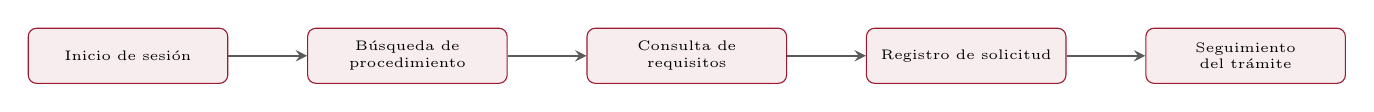
\begin{tikzpicture}[
  node distance=1.0cm,
  box/.style={
    draw=unsaacRed, fill=unsaacRed!8, rounded corners=3pt,
    text width=2.3cm, align=center, font=\tiny, minimum height=0.7cm
  },
  arr/.style={->, >=stealth, draw=unsaacGray, thick}
]
  \node[box] (A) {Inicio de sesión};
  \node[box, right=of A] (B) {Búsqueda de procedimiento};
  \node[box, right=of B] (C) {Consulta de requisitos};
  \node[box, right=of C] (D) {Registro de solicitud};
  \node[box, right=of D] (E) {Seguimiento del trámite};
  \draw[arr] (A)--(B);
  \draw[arr] (B)--(C);
  \draw[arr] (C)--(D);
  \draw[arr] (D)--(E);
\end{tikzpicture}
\end{center}

\medskip
\textbf{Flujo del administrador:}

\begin{center}
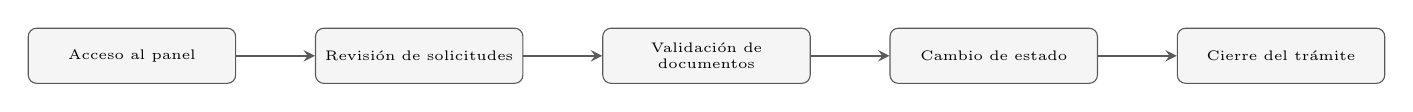
\begin{tikzpicture}[
  node distance=1.0cm,
  box/.style={
    draw=unsaacGray, fill=lightGray, rounded corners=3pt,
    text width=2.4cm, align=center, font=\tiny, minimum height=0.7cm
  },
  arr/.style={->, >=stealth, draw=unsaacGray, thick}
]
  \node[box] (A) {Acceso al panel};
  \node[box, right=of A] (B) {Revisión de solicitudes};
  \node[box, right=of B] (C) {Validación de documentos};
  \node[box, right=of C] (D) {Cambio de estado};
  \node[box, right=of D] (E) {Cierre del trámite};
  \draw[arr] (A)--(B);
  \draw[arr] (B)--(C);
  \draw[arr] (C)--(D);
  \draw[arr] (D)--(E);
\end{tikzpicture}
\end{center}

\subsubsection{Alcance dentro del primer entregable}

En el marco del presente primer entregable, el prototipo dinámico se presenta como
una propuesta inicial de diseño que acompaña al plan de proyecto. Su alcance incluye:

\begin{itemize}
  \item La definición de la paleta de colores, tipografía y guía de estilo visual de
        la plataforma, con identidad afín a los colores institucionales de la UNSAAC.
  \item El diseño de las vistas descritas en la tabla anterior, con navegación funcional
        entre pantallas mediante los prototipos interactivos de Figma.
  \item La representación del flujo principal del usuario estudiante y del flujo del
        administrador, tal como se detallan en los diagramas anteriores.
\end{itemize}

El prototipo no constituye la implementación final de la plataforma; su función es
servir como artefacto de comunicación y validación entre el equipo de desarrollo, el
docente y los usuarios potenciales, sentando las bases para el diseño definitivo que
se elaborará en el segundo entregable semestral.

\subsubsection{Enlace al prototipo}

\begin{supuesto}
\small\textbf{Propuesta inicial:} El enlace al prototipo interactivo en Figma será
incluido aquí una vez concluido su diseño. Se recomienda publicarlo en modalidad
\emph{View Only} para facilitar la revisión por parte del docente y los usuarios
de prueba:\\[4pt]
\texttt{[Enlace al prototipo Figma --- por completar antes de la entrega formal]}
\end{supuesto}

% ── Base de Datos ────────────────────────────────────────────────────────────
\section{Base de Datos}

\subsection{Descripción general}

El diseño de la base de datos responde directamente a los requerimientos funcionales
identificados en el Sprint~1. Se optó por un modelo relacional implementado en
\textbf{PostgreSQL}, sistema gestor que ofrece soporte robusto para integridad
referencial, consultas complejas y transacciones seguras, características
indispensables para la gestión de trámites administrativos en una institución del
tamaño de la UNSAAC.

El modelo contempla once tablas que representan las entidades del dominio del problema:
especialidades, usuarios generales, usuarios administrativos, categorías, trámites,
requisitos, solicitudes, documentos, observaciones, seguimiento y notificaciones. Una
decisión de diseño central es la separación de los actores del sistema en dos tablas
independientes ---\texttt{usuario\_general} y \texttt{usuario\_admin}---, lo que
simplifica el control de acceso y refleja con claridad la distinción funcional entre
quienes realizan trámites y quienes los gestionan. Las relaciones entre las entidades
reproducen los flujos administrativos reales de la institución, desde la consulta del
catálogo del TUPA hasta la resolución y cierre de cada trámite.

\subsection{Diagrama Entidad-Relación}

A continuación se presenta el Diagrama Entidad-Relación (DER) del sistema, que ilustra
las entidades definidas, sus atributos principales y las relaciones entre ellas:

\begin{figure}[H]
  \centering
  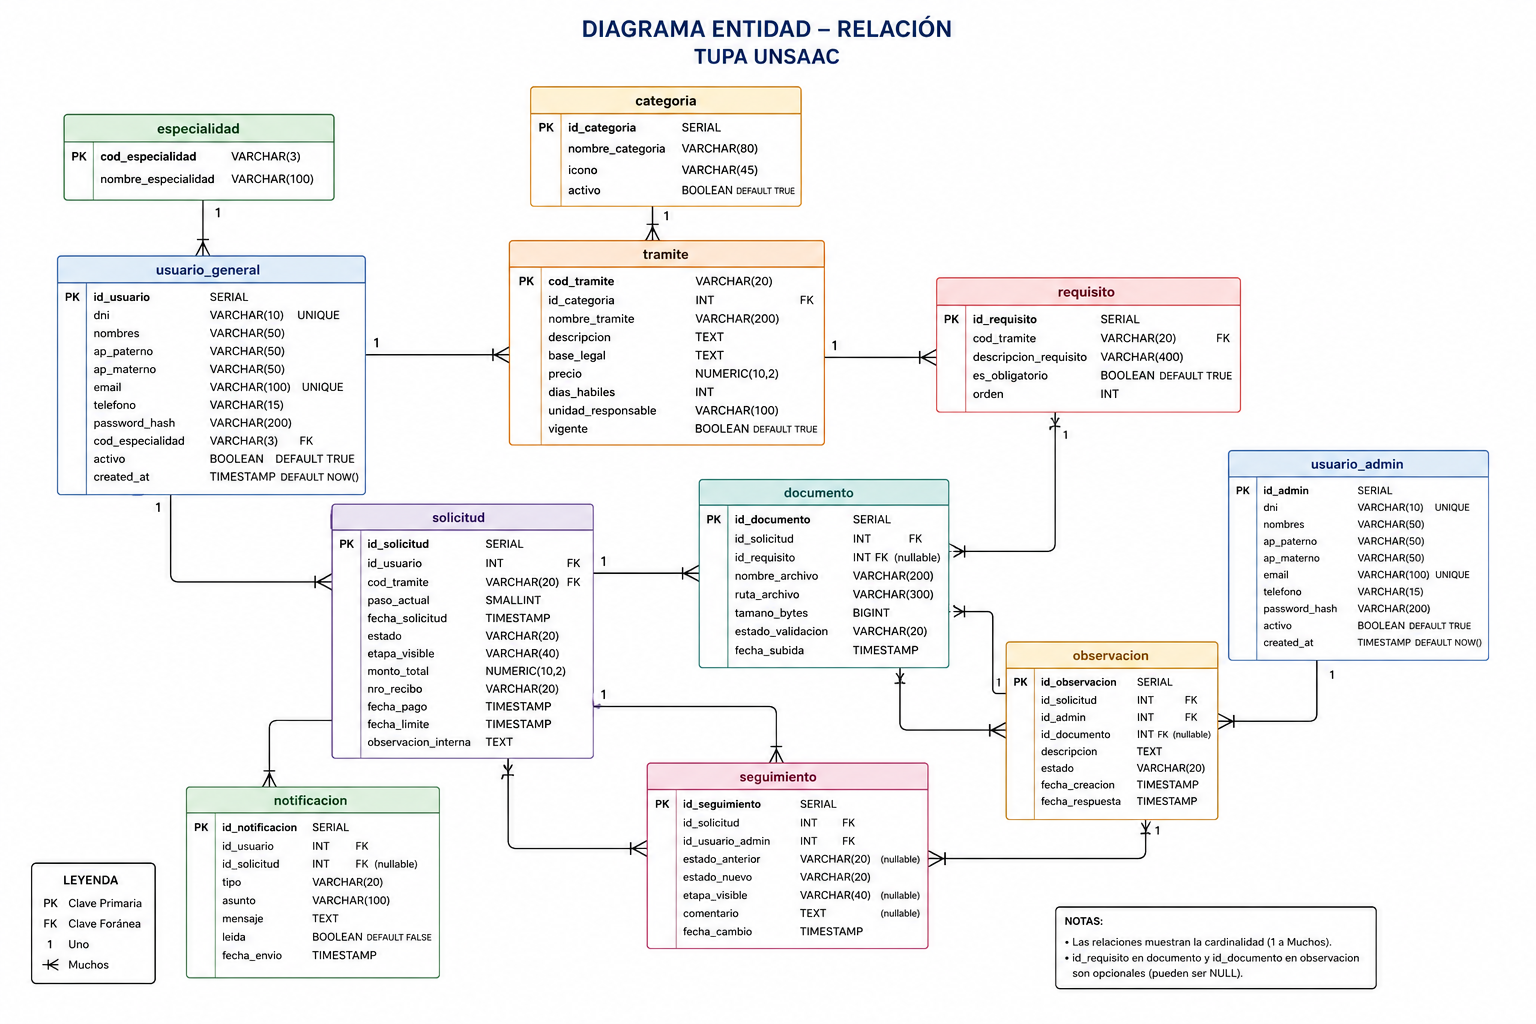
\includegraphics[width=0.9\textwidth]{images/DiagramaEntidadRelacion.png}
  \caption{Diagrama Entidad-Relación del sistema TUPA-UNSAAC}
  \label{fig:der-sistema}
\end{figure}

\subsection{Descripción de las entidades}

El modelo de datos está compuesto por las siguientes once entidades:

\begin{itemize}
  \item \textbf{Especialidad (\texttt{especialidad}):} catálogo de carreras y escuelas
        profesionales de la UNSAAC, identificadas por un código de tres caracteres
        (\texttt{cod\_especialidad}). Permite vincular a cada usuario general con su
        programa académico correspondiente.

  \item \textbf{Usuario General (\texttt{usuario\_general}):} almacena la información
        de los usuarios que realizan trámites ante la universidad. Registra DNI, nombres,
        apellidos, correo electrónico, teléfono, credenciales de acceso y la especialidad
        académica a la que pertenecen. Estos usuarios pueden consultar el catálogo del
        TUPA, iniciar solicitudes a través del wizard de seis pasos, cargar documentos y
        dar seguimiento al estado de sus trámites.

  \item \textbf{Usuario Admin (\texttt{usuario\_admin}):} representa al personal
        administrativo del sistema. Registra los mismos datos personales y de
        autenticación que el usuario general, pero sin vinculación a una especialidad
        académica. Los administradores revisan solicitudes, validan documentos, emiten
        observaciones, cambian estados de trámites y consultan los indicadores de gestión
        del panel administrativo.

  \item \textbf{Categoría (\texttt{categoria}):} agrupa los trámites del TUPA en
        clasificaciones temáticas (Académicos, Facultad, Investigación, Bienestar,
        entre otros) para facilitar la navegación y filtrado en el catálogo público.
        Incluye un atributo de ícono para su representación visual en la interfaz.

  \item \textbf{Trámite (\texttt{tramite}):} tabla central del catálogo público,
        representa cada uno de los procedimientos contemplados en el TUPA vigente.
        Registra el código del trámite, su nombre, descripción, base legal que lo
        sustenta, precio, plazo de atención en días hábiles, unidad orgánica responsable
        y estado de vigencia. Cada trámite pertenece a una categoría.

  \item \textbf{Requisito (\texttt{requisito}):} documenta las condiciones y documentos
        necesarios para iniciar cada trámite. Cada requisito está vinculado a un trámite
        específico e incluye su descripción, carácter obligatorio u opcional y un orden
        de presentación. Se muestra tanto en el catálogo público como en el paso~3 del
        wizard de solicitud.

  \item \textbf{Solicitud (\texttt{solicitud}):} entidad central del ciclo de vida de
        un trámite, registra cada procedimiento iniciado por un usuario general. Gestiona
        el estado interno del proceso (\texttt{BORRADOR}, \texttt{SOLICITADO},
        \texttt{EN~PROCESO}, \texttt{PAGADO}, \texttt{SUBSANACION}, \texttt{COMPLETADO}
        o \texttt{ANULADO}), la etapa visible en la línea de tiempo, el paso actual del
        wizard (1~a~6, con restricción \texttt{CHECK}), las fechas relevantes, el monto
        total, el número de recibo y los datos de pago asociados.

  \item \textbf{Documento (\texttt{documento}):} almacena las referencias a los archivos
        digitales que el usuario carga durante el paso~3 del wizard. Cada documento se
        vincula a la solicitud correspondiente y al requisito específico que cubre,
        registrando el nombre del archivo, su ruta en el servidor, tamaño en bytes y
        estado de validación (\texttt{PENDIENTE}, \texttt{APROBADO} o
        \texttt{RECHAZADO}).

  \item \textbf{Observación (\texttt{observacion}):} registra las incidencias señaladas
        por un administrador sobre documentos específicos de una solicitud. Cuando un
        documento presenta un problema, el administrador emite una observación con la
        descripción del defecto detectado, vinculada al documento en cuestión. El estado
        de la solicitud cambia automáticamente a \texttt{SUBSANACION} y se genera una
        notificación al usuario para que corrija y vuelva a cargar la documentación.
        La observación puede pasar por los estados \texttt{PENDIENTE},
        \texttt{SUBSANADO} y \texttt{CERRADO}.

  \item \textbf{Seguimiento (\texttt{seguimiento}):} log de auditoría que registra de
        forma cronológica todos los cambios de estado de una solicitud. Cada entrada
        almacena el estado anterior, el estado nuevo, la etapa visible correspondiente,
        un comentario opcional y la referencia al administrador que ejecutó el cambio.
        Esta tabla alimenta la línea de tiempo visual del módulo de seguimiento del
        usuario.

  \item \textbf{Notificación (\texttt{notificacion}):} registra las alertas enviadas
        automáticamente a los usuarios generales ante eventos relevantes: cambios de
        estado (\texttt{ESTADO}), observaciones emitidas (\texttt{OBSERVACION}),
        verificación de pagos (\texttt{PAGO}) o proximidad de vencimiento
        (\texttt{VENCIMIENTO}). Cada notificación incluye asunto, mensaje, indicador
        de lectura y la solicitud asociada.
\end{itemize}

\subsection{Consideraciones de diseño}

El modelo adopta las siguientes decisiones de diseño relevantes:

\begin{itemize}
  \item La separación de usuarios en dos tablas independientes
        ---\texttt{usuario\_general} y \texttt{usuario\_admin}--- responde a la
        distinción funcional clara entre los actores del sistema: los usuarios generales
        inician y dan seguimiento a trámites, mientras que los administradores gestionan,
        validan y resuelven solicitudes. Esta separación simplifica las consultas, evita
        columnas nulas innecesarias (como \texttt{cod\_especialidad} para
        administradores) y facilita la implementación de políticas de acceso
        diferenciadas en el backend.

  \item Los documentos adjuntos se almacenan como referencias a rutas de archivos en el
        servidor (atributo \texttt{ruta\_archivo}), no como datos binarios en la base de
        datos, lo que optimiza el rendimiento de las consultas y facilita la gestión
        independiente del almacenamiento.

  \item La tabla \texttt{seguimiento} se mantiene como entidad independiente para
        garantizar la trazabilidad completa del ciclo de vida de cada trámite sin
        modificar los registros originales de la solicitud, respetando principios básicos
        de auditoría de datos y permitiendo reconstruir la línea de tiempo completa de
        cualquier procedimiento.

  \item El sistema distingue entre el \textbf{estado interno} de una solicitud (utilizado
        por la lógica de negocio: \texttt{BORRADOR}, \texttt{SOLICITADO}, etc.) y la
        \textbf{etapa visible} (texto mostrado al usuario en la línea de tiempo:
        \emph{Recibido}, \emph{Evaluación técnica}, \emph{Pago verificado}, etc.), lo
        que permite adaptar la comunicación al usuario sin alterar la máquina de estados
        del proceso administrativo.

  \item Se definieron índices sobre las columnas de consulta más frecuente ---DNI, email,
        estado de solicitud, fecha, relaciones foráneas y notificaciones no leídas---
        para optimizar el rendimiento de las operaciones de búsqueda y filtrado en los
        módulos de catálogo, seguimiento y panel administrativo.
\end{itemize}

\subsection{Relaciones entre entidades}

Las relaciones principales del modelo se resumen a continuación:

\begin{itemize}
  \item \texttt{especialidad} $\rightarrow$ \texttt{usuario\_general}: una especialidad
        puede tener múltiples usuarios generales asociados.
  \item \texttt{categoria} $\rightarrow$ \texttt{tramite}: cada categoría agrupa
        múltiples trámites del catálogo.
  \item \texttt{tramite} $\rightarrow$ \texttt{requisito}: cada trámite define uno o
        más requisitos documentales.
  \item \texttt{usuario\_general} y \texttt{tramite} $\rightarrow$ \texttt{solicitud}:
        cada solicitud vincula a un usuario general con un trámite específico.
  \item \texttt{solicitud} y \texttt{requisito} $\rightarrow$ \texttt{documento}: cada
        documento cargado se asocia a una solicitud y al requisito que cubre.
  \item \texttt{solicitud} y \texttt{usuario\_admin} $\rightarrow$
        \texttt{observacion}: las observaciones son emitidas por un administrador sobre
        una solicitud, vinculadas opcionalmente a un documento específico.
  \item \texttt{solicitud} y \texttt{usuario\_admin} $\rightarrow$
        \texttt{seguimiento}: cada cambio de estado es registrado por un administrador
        como entrada de auditoría.
  \item \texttt{usuario\_general} y \texttt{solicitud} $\rightarrow$
        \texttt{notificacion}: las notificaciones se dirigen a un usuario general y se
        asocian a una solicitud.
\end{itemize}

\begin{figure}[H]
  \centering
  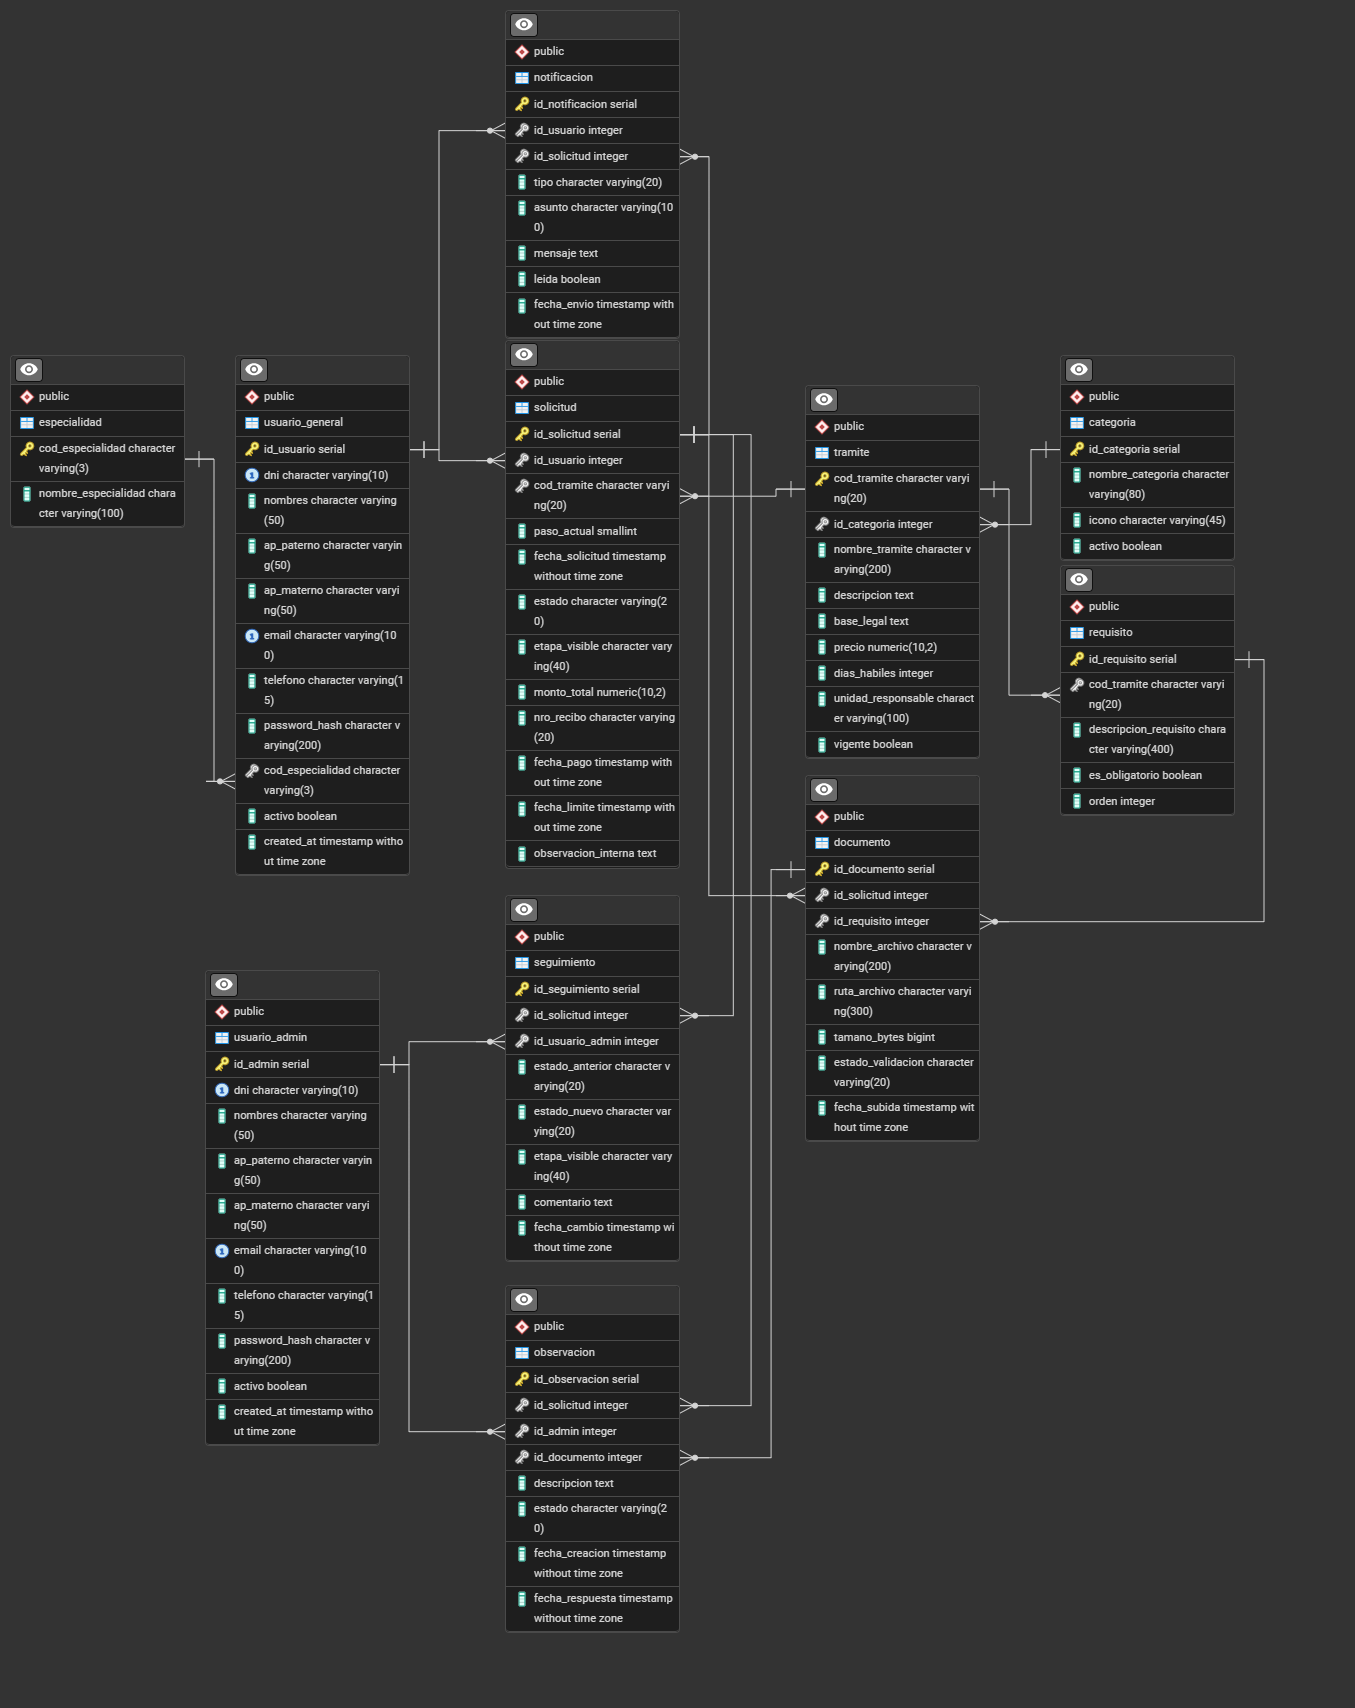
\includegraphics[width=0.9\textwidth]{images/BDDDiagram.png}
  \caption{Modelo relacional de la base de datos --- diagrama físico}
  \label{fig:modelo-relacional}
\end{figure}


%% BIBLIOGRAFÍA
\printreferences[Referencias Bibliográficas]

\end{document}
